% \section{Disentangled Representation}
\paragraph{Local Appearance Transfer.}
%More results for swapping parts on the Deep Fashion dataset are shown in Fig.~\ref{fig:partswaps}, as an extension to main paper, Fig. 8. The full range of possibilities for swapping part-wise appearance and body pose is best viewed in the attached video (parttransfer.mp4).
In Fig.~\ref{fig:partswaps}, we show  results for successively swapping part appearance on the Deep Fashion dataset.
% The full range of possibilities for swapping part-wise appearance and shape is best viewed in the attached video (localtransfer.mp4).

\paragraph{Video-to-Video Translation.}
In Fig.~\ref{fig:bbc1} we show sequences of a frame-to-frame appearance-shape transfer on the BBC Pose dataset. Note that the out-of-plane rotations and fine-grained details of hands and facial expressions are accurately captured. Notice the quality (smoothness, consistency) of the transfer.
% becomes most prominent in the provided video (vid2vid.mp4).
%
\begin{figure}[b!]
    \vspace*{-1.em}
	\centering
	\begin{subfigure}{.43\linewidth}
	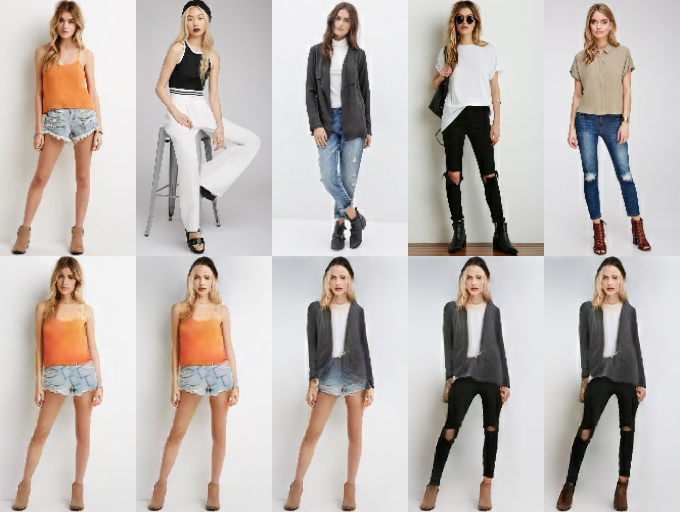
\includegraphics[trim={0cm 0cm 0cm 0cm},clip, width=1.\linewidth]{fig/supp/DeepF/1}
	\label{fig:part3_21}
	\end{subfigure}\hspace{0.03\textwidth}
	\vspace*{-1.em}
	\centering
	\begin{subfigure}{.43\linewidth}
	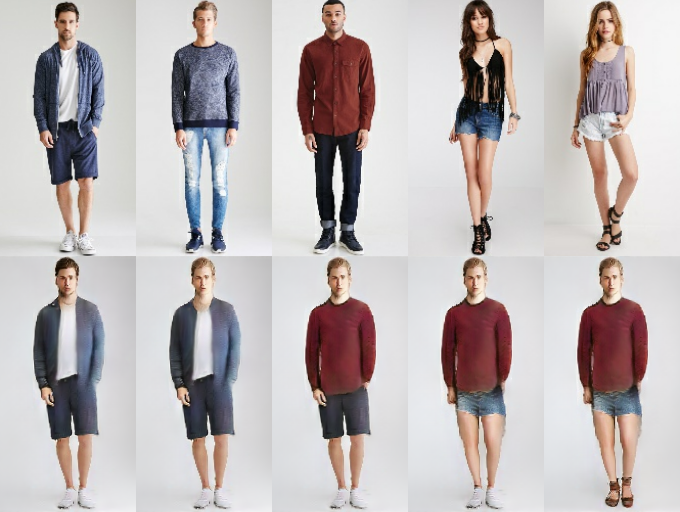
\includegraphics[trim={0cm 0cm 0cm 0cm},clip, width=1.\linewidth]{fig/supp/DeepF/6}
	\label{fig:part3_30}
	\end{subfigure}
	\vspace*{-1.em}
	\centering
	\begin{subfigure}{.43\linewidth}
	\centering
	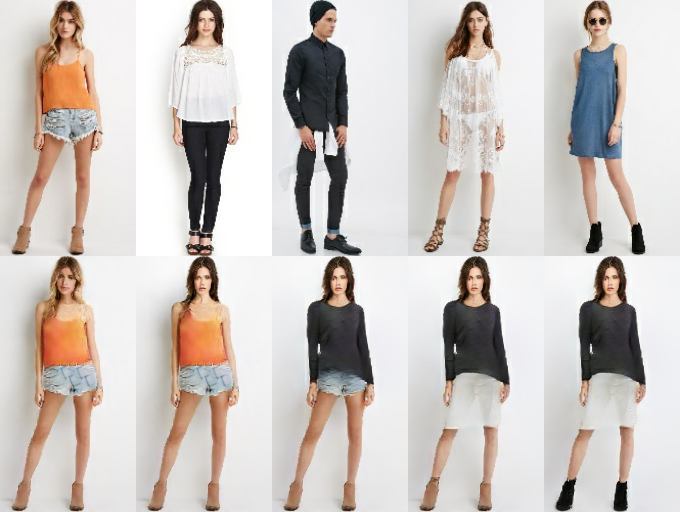
\includegraphics[trim={0cm 0cm 0cm 0cm},clip, width=1.\linewidth]{fig/supp/DeepF/2}
	\label{fig:part3_30}
	\end{subfigure}\hspace{0.03\textwidth}
	\label{fig:partswaps2}
	\centering
	\begin{subfigure}{.43\linewidth}
	\centering
	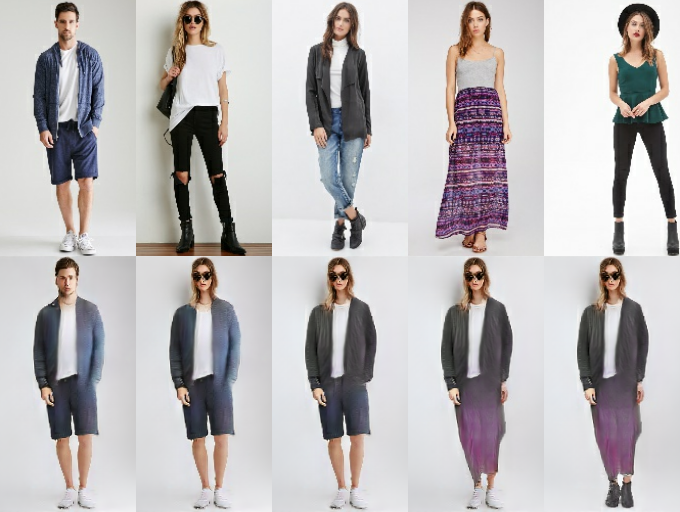
\includegraphics[trim={0cm 0cm 0cm 0cm},clip, width=1.\linewidth]{fig/supp/DeepF/4}
	\label{fig:part3_21}
	\end{subfigure}
	\centering
	\begin{subfigure}{.43\linewidth}
	\centering
	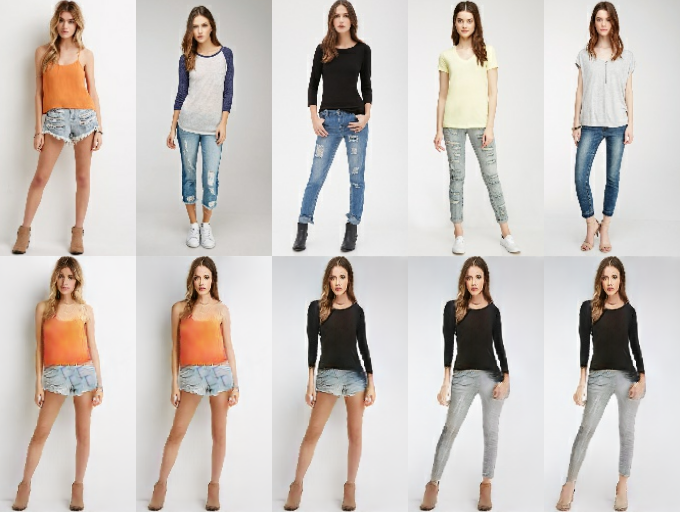
\includegraphics[trim={0cm 0cm 0cm 0cm},clip, width=1.\linewidth]{fig/supp/DeepF/3}
	\label{fig:part3_30}
	\end{subfigure}\hspace{0.03\textwidth}
	\centering
	\begin{subfigure}{.43\linewidth}
	\centering
	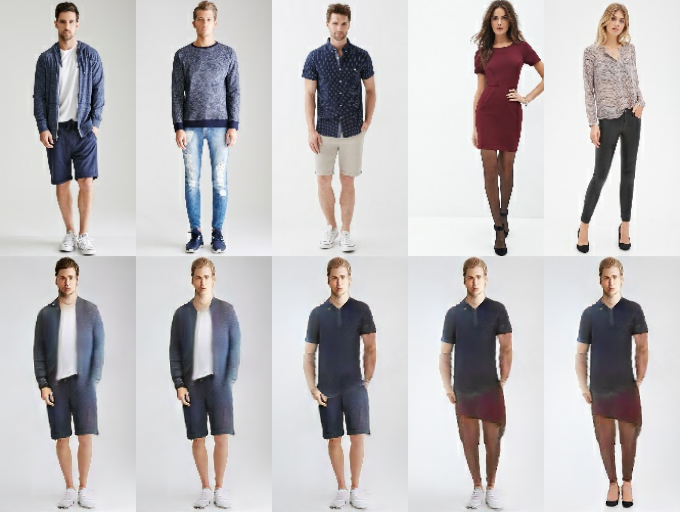
\includegraphics[trim={0cm 0cm 0cm 0cm},clip, width=1.\linewidth]{fig/supp/DeepF/7}
	\label{fig:part3_30}
	\end{subfigure}
	\caption{
	Successively altering the appearance of individual parts. We show 6 examples of successively altering appearances of parts using different source images. In each example we start from the original appearance (left-most column). The top row shows ground-truth images (taken from the test-set), which act as the source for the part appearance to be altered. The bottom row then illustrates the new synthesized image, which is generated based on the already altered part appearances plus the current appearance modification. Part appearances are altered in fixed order: head, upper body, legs, feet.
	}
	\label{fig:partswaps}
\end{figure}
% \newpage

\begin{figure}[b!]
	\centering
	% \begin{subfigure}{.49\linewidth}
	\centering
	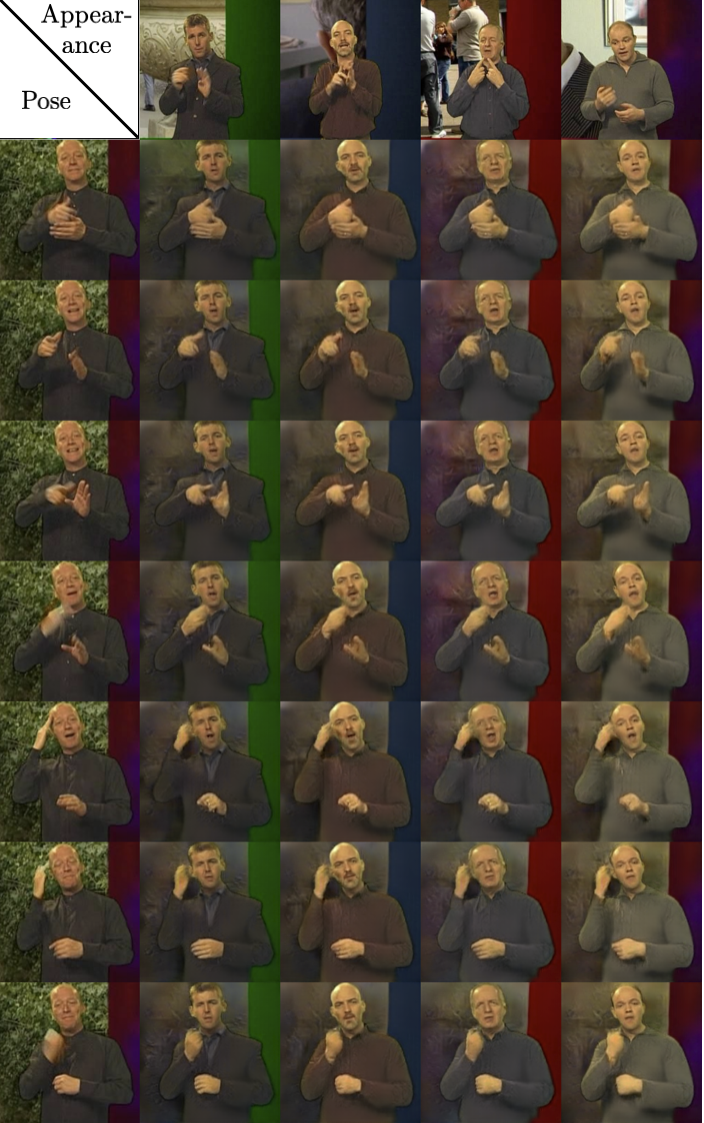
\includegraphics[trim={0cm 0cm 0cm 0cm},clip, width=.8\linewidth]{fig/supp/bbc}
	% \end{subfigure}\hspace{0.01\textwidth}
	% \centering
	% \begin{subfigure}{.49\linewidth}
	% \centering
	% 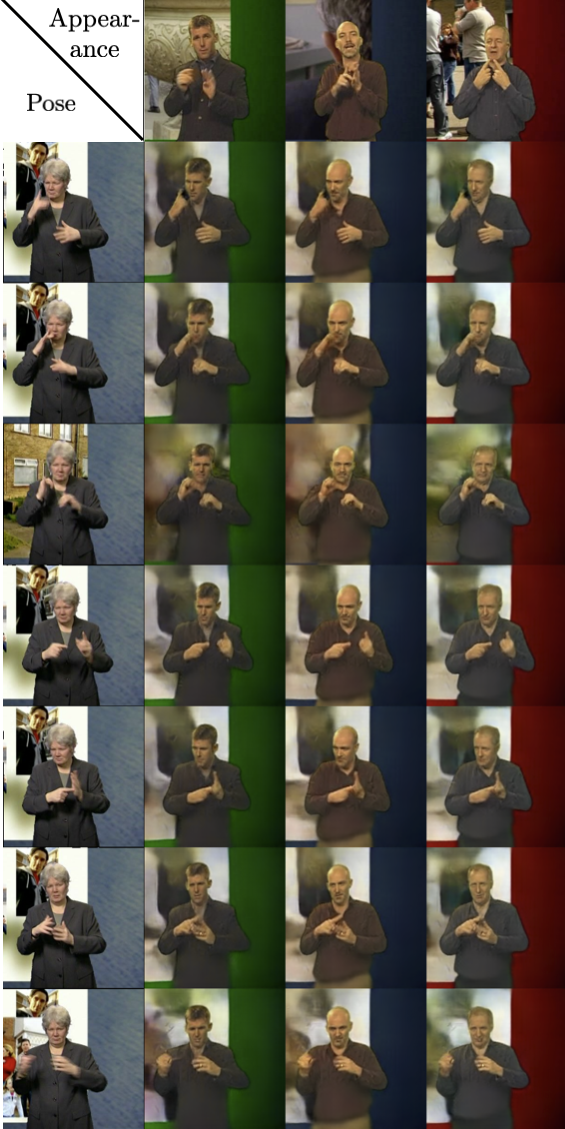
\includegraphics[trim={0cm 0cm 0cm 0cm},clip, width=1.\linewidth]{fig/supp/bbc_new2}
	% \end{subfigure}
	\caption{Generated sequence on BBC Pose from a target pose sequence (leftmost column) and target appearances (top row). }
	\label{fig:bbc1}
\end{figure}


